\chapter{Inferspark-Graph}
\label{chap:graphengine}

Although InferSpark has achieved good scalability compared to the existing
probabilistic programming frameworks, InferSpark still suffers from poor
performance when the data size increases. In this
chapter, we first identify the cause of the poor performance. It turns out to be a
limitation of the physical design of GraphX. The problem has not been addressed
before because it has a much less significant impact on performance of the
existing applications (e.g. PageRank) than the VMP algorithm in InferSpark.
Then we propose a new physical design to solve the problem. Finally, we
present our implementation, InferSpark-Graph, and an empirical evaluation to
show its improvement of the performance of InferSpark.

\section{Cause of Poor Performance}
\label{sec:cause_poor_perf}

In the Spark Web UI, we find there are some workers spending majority of their 
running time in writing out data or waiting for remote data. The poor
performance is primarily caused by the slow data shuffle.

Data shuffle is an expensive operation in a distributed system because it
involves a lot of random disk I/Os and large amount of network traffic between each
pair of workers. In the case of Apache Spark, either slow random disk I/O or
low network bandwidth is a bottleneck of the shuffle performance. In most
cases, the random I/O is the main contributing factor to the poor shuffle
performance although shuffle file consolidation mitigates the problem
\sjtucite{spark-shuffle}. Our cluster is configured so that the network
bandwidth is roughly the same as the sequential disk I/O speed. Hence, the 10x
slower random I/O becomes a major bottleneck in the system when there is large
amount of shuffle between each pair of workers.
In order to verify that random I/O is the major bottleneck, 
we use a Ganglia server to monitor the runtime metrics including CPU usage,
memory, disk I/O, network, Java garbage collection performance. We find disk
I/O pattern matches the case where random I/O is the bottleneck. We also rules
out other factors such as java GC since they do not take a majority of the
running time. Therefore, we conclude that the poor performance arises from the
excessive amount of data shuffle during graph update in each substep of the VMP
algorithm. In order to solve the problem, we analyze the shuffle stages in
each substep and identify ways to reduce the amount of shuffle.

\begin{figure}[h]
\centering
\begin{lstlisting}
val prevg = g
val activeSet = g.vertices.filter(isActiveVertex)
val msg = g.aggregateMessages(sendFunc, mergeFunc, TripletFields, activeSet, edgeDirection)
g = g.outerJoinVertices(msg)(updateFunc).persist()
g.edges.count()
prevg.unpersist()
\end{lstlisting}
\caption{The actual code for a substep of the VMP algorithm}
\label{fig:code_substep_actual}
\end{figure}

Consider a substep of the VMP algorithm (see \figref{fig:code_substep_actual}).
Note that the code shown above is slightly different from
\figref{fig:code_substep}. We use an additional active set to specify
which vertices are active in our actual implementation. A substep expands to 3
shuffle stages (see \figref{fig:graphx_substep}) and an result stage in GraphX.

\begin{figure}[t]
	\centering
	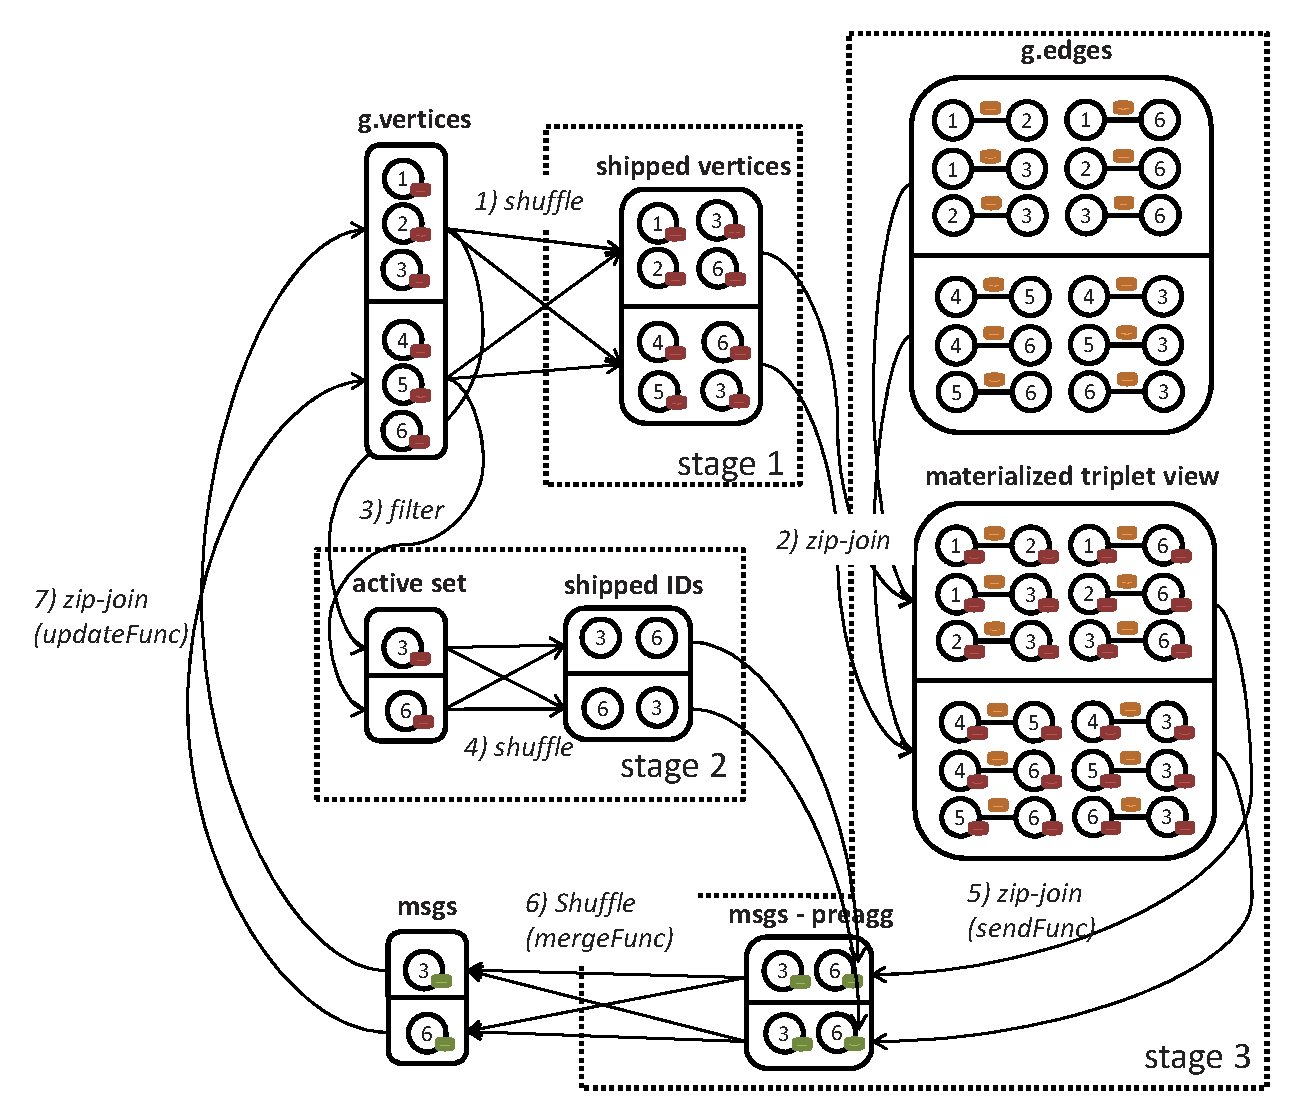
\includegraphics[scale=0.5,clip]{figs/graphx_substep.eps}
	\caption{Stages of a substep in GraphX}
	\label{fig:graphx_substep}
\end{figure}

\begin{itemize}
	\item Shuffle stage 1
		\begin{itemize}
			\item[1)] Shuffle vertex attributes to the edge partitions.
		\end{itemize}

	\item Shuffle stage 2
		\begin{itemize}
			\item[3)] Filter out active vertices from vertex RDD to form the active set.
			\item[4)] Shuffle the IDs in the active set to the edge partitions.
		\end{itemize}

	\item Shuffle stage 3
		\begin{itemize}
			\item[2)] Zip-join shipped vertex attributes with the edge partitions in
				order to maintain the triplet view.
			\item[5)] Zip-join the triplet view with shipped vertices and run
				``sendFunc'' on each active edge. Do partial aggregation on the messages
				using ``mergeFunc'' to get the ``msgs - preagg'' RDD.
			\item[6)] Shuffle the messages and complete the aggregations using
				``mergeFunc''. The resulting ``msg'' RDD is co-partitioned with the
				vertex partition.
		\end{itemize}

	\item Result stage
			\begin{itemize}
				\item[7)] Zip-join ``msgs'' with the vertex RDD and run ``updateFunc'' on
					the vertices that receive messages. The new vertex RDD is then
					persisted in the memory.
			\end{itemize}

\end{itemize}

Among all the three shuffle stages, the shuffle sizes of stage 1 and 3 are the
largest. The shuffle size of stage 1 is the size of vertices that is updated
and need to be replicated to the edge partitions. In the case of VMP,
the size is quite large since either the vertex attributes are very large data
structure, the number of vertices updated is
proportional to the number of words in a corpus, or both. The shuffle size of
stage 3 is the size of messages sent along the edges in a substep. The
messages are similar to the replicated vertices in that they are either very
large, of a large amount or both. 

The way that GraphX implements data shuffle is to simply re-partition the
vertices or messages according to the partitioner of the RDD to be
zip-joined with uses. Take stage 1 as an example. GraphX first flat maps each
vertex partition $i$ to an array of vertex blocks. The vertices in block $j$
are the vertices that need to be replicated in
edge partition $j$.  Block $j$ is also paired
with the partition ID $j$ so that it can be re-partitioned using the edge
RDD's partitioner. Finally, GraphX calls ``partitionBy'' on the resulting RDD
to get an RDD of replicated vertices that is zip-joinable with the edge RDD.

The problem is that the vertices are nevertheless shuffled even if almost all
the vertices in the same vertex partition will be replicated in the same edge
partition. If almost all the vertices in a vertex partition are sent to the
same edge partition, we call the latter the \emph{corresponding} edge
partition of the vertex partition. That is, however, exactly the case using
InferSpark's partition strategy in all substeps where about $\frac{2}{2}$ of
the vertices need to be shipped. The only substep where vertices are sent to
all the edge partitions only sends a small constant number of vertices. Hence,
almost all shuffle can be avoided if vertices can be sent to the corresponding
edge partition without shuffle. 

Assuming that the corresponding vertex partition and edge partition co-locate
on the same worker, we propose a new way of shuffling vertices to edge
partitions that optimizes away almost all shuffle in VMP:
\begin{enumerate}
	\item Identify the corresponding edge partition for each vertex partition,
		where most vertices in the vertex partition will be replicated in that
		edge partition.

	\item Filter out all the vertices that are to be replicated in other edge
		partitions for each vertex partition and shuffle them to the right
		partition.

	\item Zip-join the original vertex RDD, the shuffled vertices and the edge
		RDD. 
\end{enumerate}

\section{InferSpark-Graph Solution}
\label{sec:inferspark_graph_solution}

Implementing the optimization describe in Section \ref{sec:cause_poor_perf}
requires three major changes to the GraphX implementation and InferSpark
CodeGen module implementation:
\begin{itemize}
	\item InferSpark CodeGen module has to generate vertex partitioner which
		partitions vertices in such a way that corresponding vertex partition and
		edge partition share the same partition ID. This is already implemented in
		InferSpark.

	\item We need to re-implement the shuffle in GraphX in the way described in
		Section \ref{sec:cause_poor_perf}.

	\item We need to ensure that the corresponding vertex and edge partitions
		co-locate on the same worker. This is, however, {\tt not possible} with
		the separate vertex and edge RDD design in GraphX. Spark assigns a
		partition to any of the free workers at time of task scheduling. When
		the vertex RDD and edge RDD are being built, the partitions with the same
		ID could be assigned to different workers. In the subsequent iterations,
		the partitions will probably remain their initial location due to
		locality.
\end{itemize}

\begin{figure}
	\centering
	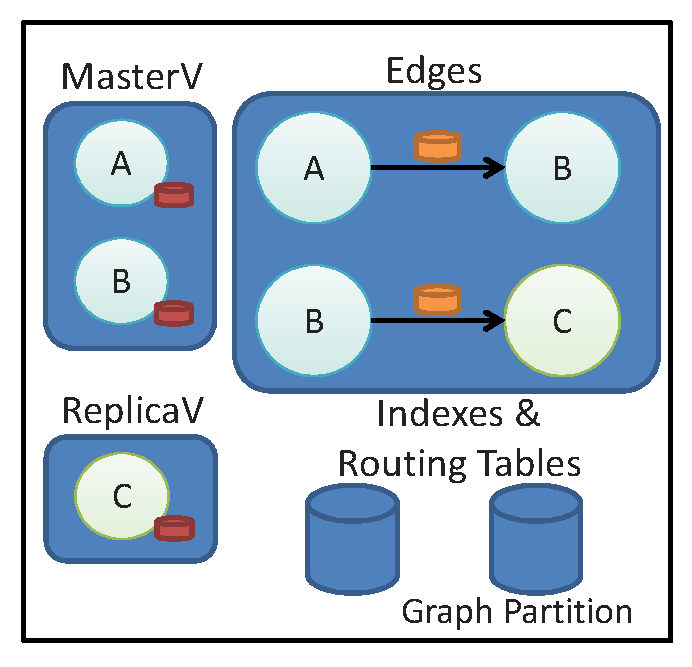
\includegraphics[scale=0.5,clip]{figs/graph_partition.eps}
	\caption{Design of a graph partition}
	\label{fig:inferspark_graph_partition}
\end{figure}

The only way to overcome the third limitation is to create a new graph processing
framework, InferSpark-Graph. It merges corresponding vertex partition and
edge partition into one single partition. We call the merged partition a graph
partition. Thus, the corresponding partitions co-locate on the same worker
since they are bundled together. We also notice that the those vertices in a
vertex partition that are replicated in the corresponding partition are now
duplicates in the graph partition. To eliminate the duplicates, we simply drop
all the duplicate replicas. The
original copies of vertices are called the ``master'' vertices while the
replicas are called the ``replica'' vertices. All the other indexes are
retained to support efficient join and scan. The resulting graph partition
design is shown in \figref{fig:inferspark_graph_partition}.

Both InferSpark-Graph and its user have to properly persisting and
unpersisting the intermediate RDDs. For example, we cache the RDD to be joined
to the graph RDD before we split it into two parts and shuffle one of them, or
the RDD will be re-computed, incurring too much overhead. InferSpark-Graph
also has to avoid concurrent shuffle stages, which could cause some tasks to
be run on a different worker than the worker where the partition resides.
Stage 1 and Stage 2 in a substep of the VMP algorithm are a
typical example of concurrent shuffle stages. To serialize the stages, we
insert an empty action between them.

It is possible to maintain all the public API in GraphX using this new
physical design by simply flat mapping the graph partition into vertices or
edges. A more efficient way would be overriding all the API to directly
operate on the graph RDD and graph partitions. We take the second approach to
make InferSpark-Graph as efficient as possible. Existing applications of
GraphX can be ported to InferSpark-Graph by simply changing its graph
constructor from GraphX's to InferSpark-Graph's. All other public API calls
can be retained without any modification. 

For applications that share the similar characteristics like VMP in
InferSpark, i.e. the graph in those applications can be partitioned in such a
way that most vertices in a vertex partition are replicated in the same
edge partition and/or most messages sent from an edge partition are to the
same vertex partitions, the performance boost should be significant. The
characteristics are common in other inference algorithms that
we plan to support (e.g. Gibbs Sampling). As for other applications like
PageRank, where the graph cannot be partitioned that way and the
inter-partition communication is inevitable, the performance will be the same
or slightly better than using GraphX.

\section{Empirical Evaluation}

In this section, we present an empirical evaluation of the new graph
processing framework on the VMP implementation in InferSpark for LDA. We
simply switch the graph processing framework from GraphX to InferSpark-Graph
in the source code. We use the same cluster setup as the InferSpark
evaluation. All worker nodes and the master node run Linux with 2.6GHz
quad-core CPU, 32GB DRAM (22GB as executor memory), and 700GB hard disk. By
default, there are 24 workers and a master. The spark version is upgraded to
1.6.1 and the scala version is upgraded to 2.11.7. The upgrade from
spark-1.4.1 to spark-1.6.1 has no impact on the performance because the spark
core and GraphX are virtually untouched in the upgrade. The hadoop version is
2.6.0. In addition to VMP, we also runs PageRank on both GraphX and
InferSpark-Graph to verify that the performance of existing applications is the same 
or slightly better if not significantly improved.

\subsection{VMP for LDA}

We run the VMP implementation for LDA on different sizes of wikipedia dataset
using both GraphX and InferSpark-Graph for 10 iterations. The number of topics
is 96 and the vocabulary size is 9040. No checkpoint is made during the
execution. We measure the time of execution and the size of data shuffled in
each iteration.

\begin{figure*}[h]
\centering
	\subfigure[1st iteration time]{
		\label{fig:graph_cmp_first_iteration_datasize}
		\includegraphics[width=0.45\linewidth]{figs/graph_cmp_first_iteration_datasize.eps}
	}
	\subfigure[average iteration time excluding 1st iteration]{
		\label{fig:graph_cmp_average_iteration_datasize}
		\includegraphics[width=0.45\linewidth]{figs/graph_cmp_avg_iteration_datasize.eps}
	}
	\caption{Iteration time against data size of VMP for LDA using GraphX and
	InferSpark-Graph}
	\label{fig:graph_cmp_iteration_time_datasize}
\end{figure*}

\begin{figure*}[h]
\centering
	\subfigure[shuffle size]{
		\label{fig:graph_cmp_shuffle_size_datasize}
		\includegraphics[width=0.45\linewidth]{figs/graph_cmp_shuffle_size_datasize.eps}
	}
	\subfigure[total running time]{
		\label{fig:graph_cmp_total_time_datasize}
		\includegraphics[width=0.45\linewidth]{figs/graph_cmp_total_time_datasize.eps}
	}
	\caption{Total time and shuffle size against data size of VMP for LDA using GraphX and
	InferSpark-Graph}
	\label{fig:graph_cmp_shuffle_size_total_time_datasize}
\end{figure*}

\figref{fig:graph_cmp_iteration_time_datasize} shows the iteration time
comparison between GraphX and InferSpark-Graph by scaling up the data size.
Both the first iteration time and average iteration time 
using InferSpark-Graph is significantly shorter than that using
GraphX. When the data size increases, the iteration time increases linearly
using InferSpark-Graph while there is a super-linear increase of iteration
time using GraphX. It shows that InferSpark-Graph greatly improves the
scalability of InferSpark.

\figref{fig:graph_cmp_shuffle_size_datasize} shows the total size of data
shuffled among the workers in one iteration. The total size of data shuffled
using InferSpark-Graph is significantly smaller than that using GraphX. It
also reaches a fixed constant size as the data size increases in contrast of
the linear increase of the size of data shuffled using GraphX. This explains
why InferSpark-Graph could scale linearly but GraphX cannot: the shuffle in
InferSpark-Graph takes a fixed amount of time and the majority of time is
spent on computation while the shuffle in GraphX will eventually take the
majority of the time and thus incur too much system overhead.

Finally, \figref{fig:graph_cmp_total_time_datasize} shows the improvement of
total running time using InferSpark-Graph. Though the total running time
increases super-linearly using both frameworks, the InferSpark-Graph still
runs increasingly faster than GraphX as data size increases. The
super-linearity is caused by the graph construction phase, where the size of
data shuffled is huge and inevitable.

\subsection{Existing Application: PageRank}

We run the PageRank application in the GraphX package using both
InferSpark-Graph and GraphX for 10 iterations. The dataset is the twitter-2010
\sjtucite{BoVWFI,BRSLLP} with 41,652,230 vertices and 1,468,365,182 edges. We
then measure the running time and the size of data shuffled in each iteration.

\begin{figure*}[ht]
\centering
	\subfigure[iteration time]{
		\label{fig:pagerank_iteration_time}
		\includegraphics[width=0.45\linewidth]{figs/pagerank_iteration_time.eps}
	}
	\subfigure[shuffle size]{
		\label{fig:pagerank_shuffle_size}
		\includegraphics[width=0.45\linewidth]{figs/pagerank_shuffle_size.eps}
	}
	\caption{Iteration time and shuffle size of PageRank using GraphX and InferSpark-Graph}
	\label{fig:pagerank_perf}
\end{figure*}

\figref{fig:pagerank_perf} shows the iteration time and the size of data
shuffled in each iteration of the PageRank application using InferSpark-Graph
and PageRank. The performance of InferSpark-Graph is slightly better than
GraphX but is not much better. The reason is that the graph in PageRank is
randomly partitioned so that there are roughly the same amount of vertices
to be sent to each partition. As we claimed, InferSpark-Graph does not
improve the performance nor degrade the performance in such a case.

